\documentclass[a4paper]{article}

%% Language and font encodings
\usepackage[english]{babel}
\usepackage[utf8x]{inputenc}
\usepackage[T1]{fontenc}

%% Sets page size and margins
\usepackage[a4paper,top=3cm,bottom=2cm,left=3cm,right=3cm,marginparwidth=1.75cm]{geometry}

%% Useful packages
\usepackage{amsmath}
\usepackage{graphicx}
\usepackage[colorinlistoftodos]{todonotes}
\usepackage[colorlinks=true, allcolors=blue]{hyperref}

\usepackage{caption}
\usepackage{subcaption}

\graphicspath{{res/}}

\title{Your Paper}
\author{Lukas Finkbeiner}

\begin{document}
\maketitle

\begin{abstract}
Your abstract.
\end{abstract}

\section{Introduction}

\section{Loose Notes and Calculations}

We used one signal generator (N9310A) with a wide range of allowed frequencies, while the other (83712B) with a lower frequency limit of 10 MHz. 

We set the 83712B to run at 11 MHz and 1.5 dBm (justify??). This gave $\Delta \nu = .05 \times \nu_{LO} = .55$ MHz. We set the N9310A to run at 1.5 dBm as well and, depending on the trial, either $\nu_{RF} = \nu_{LO} + \Delta \nu = 11.55$ MHz or $\nu_{RF} = \nu_{LO} - \Delta \nu = 10.45$ MHz. 

When collecting data, we sampled at 32.5 MHz, which is more than double the Nyquist frequency. ?? why is this important and give a calculation of how far above the Nyquist this is

\

?? I didn't identify the sum and difference frequencies from observation!!

$\sin(\nu_{LO} + \Delta \nu) = \sin \nu_{LO} \cos \Delta \nu + \cos \nu_{LO} \sin \Delta \nu$

$\sin(\nu_{LO} - \Delta \nu) = \sin \nu_{LO} \cos \Delta \nu - \cos \nu_{LO} \sin \Delta \nu$

\

But these are not relevant, we want

$sin(a) + sin(a + b) = ?$, right?

$\sin(\nu_{LO}) \sin(\nu_{LO} + \Delta \nu) = \frac{1}{2} (\cos \Delta \nu - \cos (2\nu_{LO} + \Delta \nu))$ by evenness of the cosine function

and

$\sin(\nu_{LO}) \sin(\nu_{LO} - \Delta \nu) = \frac{1}{2} (\cos \Delta \nu - \cos (2\nu_{LO} - \Delta \nu))$

Why do the power spectra look the way they do. Upper sideband and lower sideband.

For the upper sideband, we can see spikes at almost the difference frequency (.575 MHz $\approx$ .55 MHz). The other spikes are at 10.2 MHz? Why?

For the lower sideband, we see outer spikes at 9 MHz. The inner spikes are still at roughly the difference frequency...

\

First I need indices of maxima?

Recreate the original using Fourier filtering. I did NOT do this!!

Explain what you see.

%Consequently, we had to establish a frequency range such that $\nu_{LO} - \Delta \nu$ would st

\section{Outline and To-Do}

Rough outline:

argue what the Nyquist criterion is, based on results.

Symmetry
* 
* Introduce correlation theorem
* Show ACF results

Observations and Data
* Include make and model of all equipment used.
* "Don't quote a number without the uncertainty and units."
* Introduce a hypothesis before each result, and justify each hypothesis with theory

% I guess ?? is now the code I use to point out areas to which I need to return later.

Discussion on results for week 2, section 1

\

I need to include details about the equipment used, but how in-depth do I need to go? Current plan
* For most things, use model number and manufacturer
* When data analysis depends on a spec sheet, offer a brief summary of the specs to which you are referring to fine-tune your analysis

\

I need uncertainties on results but I do not yet know how to get these.

\section{5}

\subsection{2}

Without taking the spectrum, we want to perform visual analysis of the plots and find periods

Motivation

* Pico sampler model, what sampling rate we used

* We're using the ugradio pico sampler code

* We're using the \_\_\_ signal generator

* Define terms $\nu_0$ = input frequency. $\nu_s$ = sampling frequency.

Finally, we took the default 16000 samples for each signal. However, for the data analysis, we will be excluding the first 100 samples due to a peculiarity of the pico sampler which distorted these (\ref{fig:pico_start}).

% Perhaps not important to discuss differences in peak to peak voltages across trials

\begin{figure}
\centering
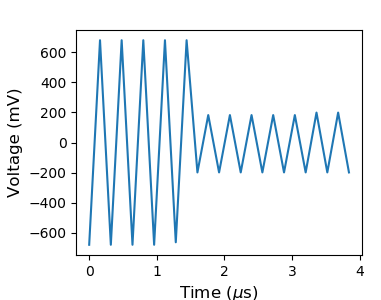
\includegraphics{pico_bad} %[width=0.3\textwidth]
\caption{\label{fig:pico_start}The oscilloscope displayed a constant signal throughout the period of data-taking. The data sampled from the pico sampler, however, reconstructs a signal with large aberrations in the first few microseconds.}
\end{figure}

\begin{figure}
\centering
\begin{minipage}{.5\textwidth}
	\centering
	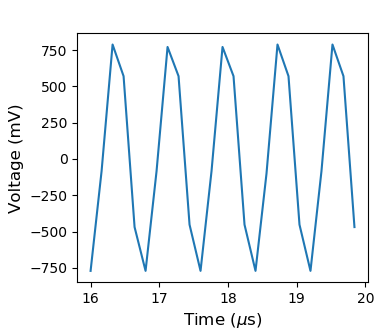
\includegraphics[width=.8\linewidth]{5-2_trial2}
	\caption{$\nu_0 = .2 \nu_s = 1.25$ MHz.}
	\label{fig:Nyq2}
\end{minipage}%
\begin{minipage}{.5\textwidth}
	\centering
	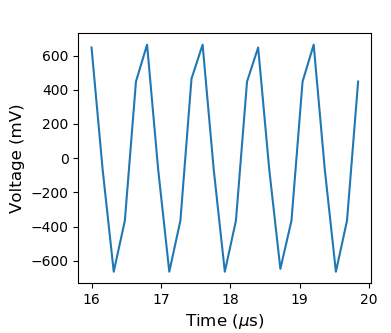
\includegraphics[width=.8\linewidth]{5-2_trial8}
	\caption{$\nu_0 = .8 \nu_s = 5$ MHz.}
	\label{fig:Nyq8}
\end{minipage}
\end{figure}

\begin{figure}
\centering
\begin{minipage}{.5\textwidth}
	\centering
	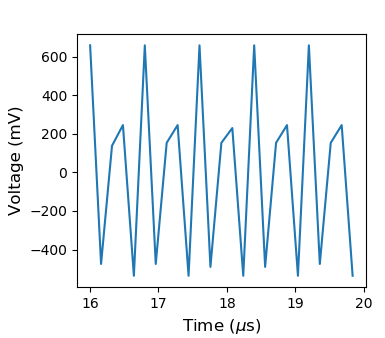
\includegraphics[width=.8\linewidth]{5-2_trial4}
	\caption{$\nu_0 = .4 \nu_s = 2.5$ MHz.}
	\label{fig:Nyq4}
\end{minipage}%
\begin{minipage}{.5\textwidth}
	\centering
	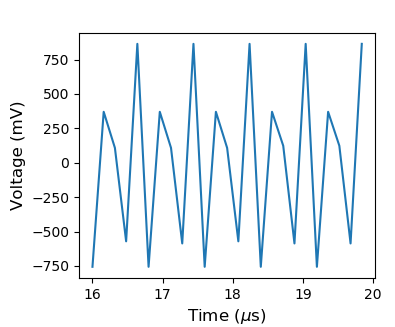
\includegraphics[width=.8\linewidth]{5-2_trial6}
	\caption{$\nu_0 = .6 \nu_s = 3.75$ MHz.}
	\label{fig:Nyq6}
\end{minipage}
\end{figure}
	
\quad We may begin inspection of the samples with a qualitative approach. Figure \ref{fig:Nyq2} shows a signal which repeats about five times in the span of about 4 microseconds. This gives us 1.25 cycles per microsecond, or 1.25 MHz, as expected. Figure \ref{fig:Nyq6} is not as obviously derived from a sine wave (the shape is distorted by the shrinking gap between $\nu_0$ and $\nu_s$), but we may still say that there is a repeating signal with slightly under five repetitions in a span of 4 microseconds. This would give us slighly under 1.25 MHz, which is incorrect; thus we have qualitatively demonstrated an aliasing effect.
% ?? Maybe I should put these annotations in the captions (it would be more appropriate there, I think)

% ?? These figures need annotations. You can probably just do the same qualitative thing that you did before.

\begin{figure}
\centering
\begin{minipage}{.5\textwidth}
	\centering
	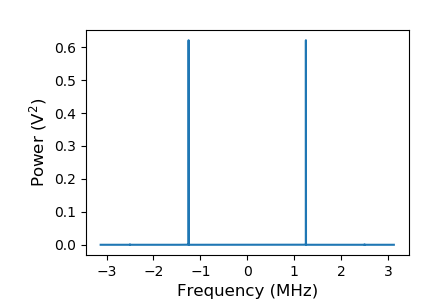
\includegraphics[width=.8\linewidth]{5-2_pow2}
	\caption{$\nu_0 = .2 \nu_s = 1.25$ MHz. Peak amplitudes at $\pm$ 1.25 MHz}
	\label{fig:NyPw2}
\end{minipage}%
\begin{minipage}{.5\textwidth}
	\centering
	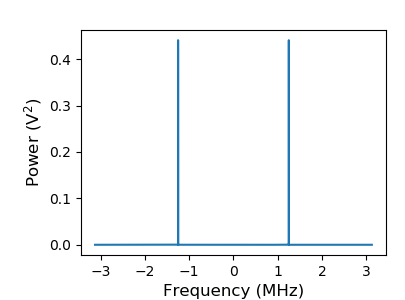
\includegraphics[width=.8\linewidth]{5-2_pow8}
	\caption{$\nu_0 = .8 \nu_s = 5$ MHz. Peak amplitudes at $\pm$ 1.25 MHz}
	\label{fig:NyPw8}
\end{minipage}
\end{figure}

\begin{figure}
\centering
\begin{minipage}{.5\textwidth}
	\centering
	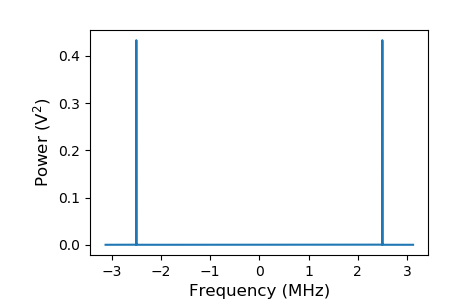
\includegraphics[width=.8\linewidth]{5-2_pow4}
	\caption{$\nu_0 = .4 \nu_s = 2.5$ MHz. Peak amplitudes at $\pm$ 2.5 MHz}
	\label{fig:NyPw2}
\end{minipage}%
\begin{minipage}{.5\textwidth}
	\centering
	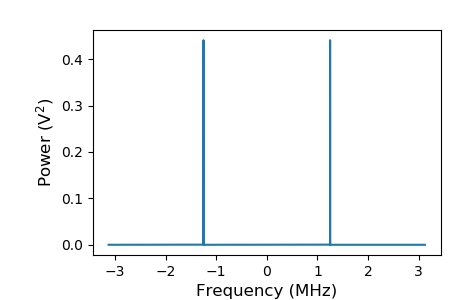
\includegraphics[width=.8\linewidth]{5-2_pow6}
	\caption{$\nu_0 = .6 \nu_s = 3.75$ MHz. Peak amplitudes at $\pm$ 2.5 MHz}
	\label{fig:NyPw8}
\end{minipage}
\end{figure}

\subsection{3}

Comments can be added to your project by clicking on the comment icon in the toolbar above. % * <john.hammersley@gmail.com> 2016-07-03T09:54:16.211Z:
%
% Here's an example comment!
%
To reply to a comment, simply click the reply button in the lower right corner of the comment, and you can close them when you're done.

Comments can also be added to the margins of the compiled PDF using the todo command\todo{Here's a comment in the margin!}, as shown in the example on the right. You can also add inline comments:

\todo[inline, color=green!40]{This is an inline comment.}

\subsection{4}

Use the table and tabular commands for basic tables --- see Table~\ref{tab:widgets}, for example. 

\begin{table}
\centering
\begin{tabular}{l|r}
Item & Quantity \\\hline
Widgets & 42 \\
Gadgets & 13
\end{tabular}
\caption{\label{tab:widgets}An example table.}
\end{table}

\subsection{5}

\LaTeX{} is great at typesetting mathematics. Let $X_1, X_2, \ldots, X_n$ be a sequence of independent and identically distributed random variables with $\text{E}[X_i] = \mu$ and $\text{Var}[X_i] = \sigma^2 < \infty$, and let
\[S_n = \frac{X_1 + X_2 + \cdots + X_n}{n}
      = \frac{1}{n}\sum_{i}^{n} X_i\]
denote their mean. Then as $n$ approaches infinity, the random variables $\sqrt{n}(S_n - \mu)$ converge in distribution to a normal $\mathcal{N}(0, \sigma^2)$.

\subsection{6}

Use section and subsections to organize your document. Simply use the section and subsection buttons in the toolbar to create them, and we'll handle all the formatting and numbering automatically.

\subsection{7}

Noise.

\section{7}

\subsection{1}

You can make lists with automatic numbering \dots

\begin{enumerate}
\item Like this,
\item and like this.
\end{enumerate}
\dots or bullet points \dots
\begin{itemize}
\item Like this,
\item and like this.
\end{itemize}

\subsection{2}

You can upload a \verb|.bib| file containing your BibTeX entries, created with JabRef; or import your \href{https://www.overleaf.com/blog/184}{Mendeley}, CiteULike or Zotero library as a \verb|.bib| file. You can then cite entries from it, like this: \cite{greenwade93}. Just remember to specify a bibliography style, as well as the filename of the \verb|.bib|.

You can find a \href{https://www.overleaf.com/help/97-how-to-include-a-bibliography-using-bibtex}{video tutorial here} to learn more about BibTeX.

We hope you find Overleaf useful, and please let us know if you have any feedback using the help menu above --- or use the contact form at \url{https://www.overleaf.com/contact}!

\subsection{3}

Single side band mixer is more difficult to perform.

\bibliographystyle{alpha}
\bibliography{sample}

\end{document}